% !TEX root = ../Diplombericht.tex
\section{Vorbereitunge RPI's}
\subsection{Betriebssystem installieren}
Für die Installation des CentOS 7.4 ist kein boot fähiger Kernel vorhanden. Das RPI kann aber dennoch mit einem Centos 7.4 betrieben werden. Dafür sind die folgenden Schritte vorzunehmen. Die Installation des Betriebssystems ist von einem Fedora Linux Client aus beschrieben.

1. Gentoo 64 Bit Image herunterladen aus dem Github Repository\footnote{\url{https://github.com/sakaki-/gentoo-on-rpi3-64bit}} von Sakaki\newline
2. Das Archiv wird mit dem Fedora Media Writer auf die SD Karte geschrieben. Dies ist anhand der Screenshots beschrieben. \newline
\begin{figure}[H]
	\centering
	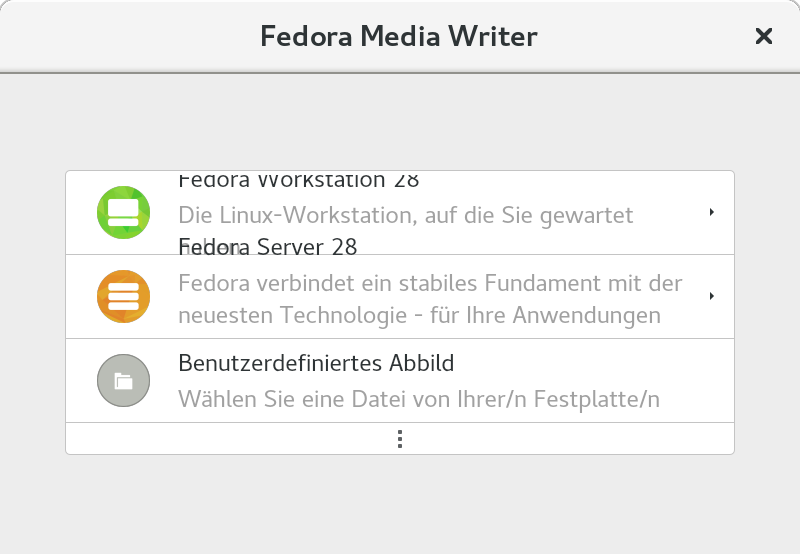
\includegraphics[scale=0.3]{Bilder/fmw1.png}
	\caption{FMW: Fedora Media Writer starten}
\end{figure}
\begin{figure}[H]
	\centering
	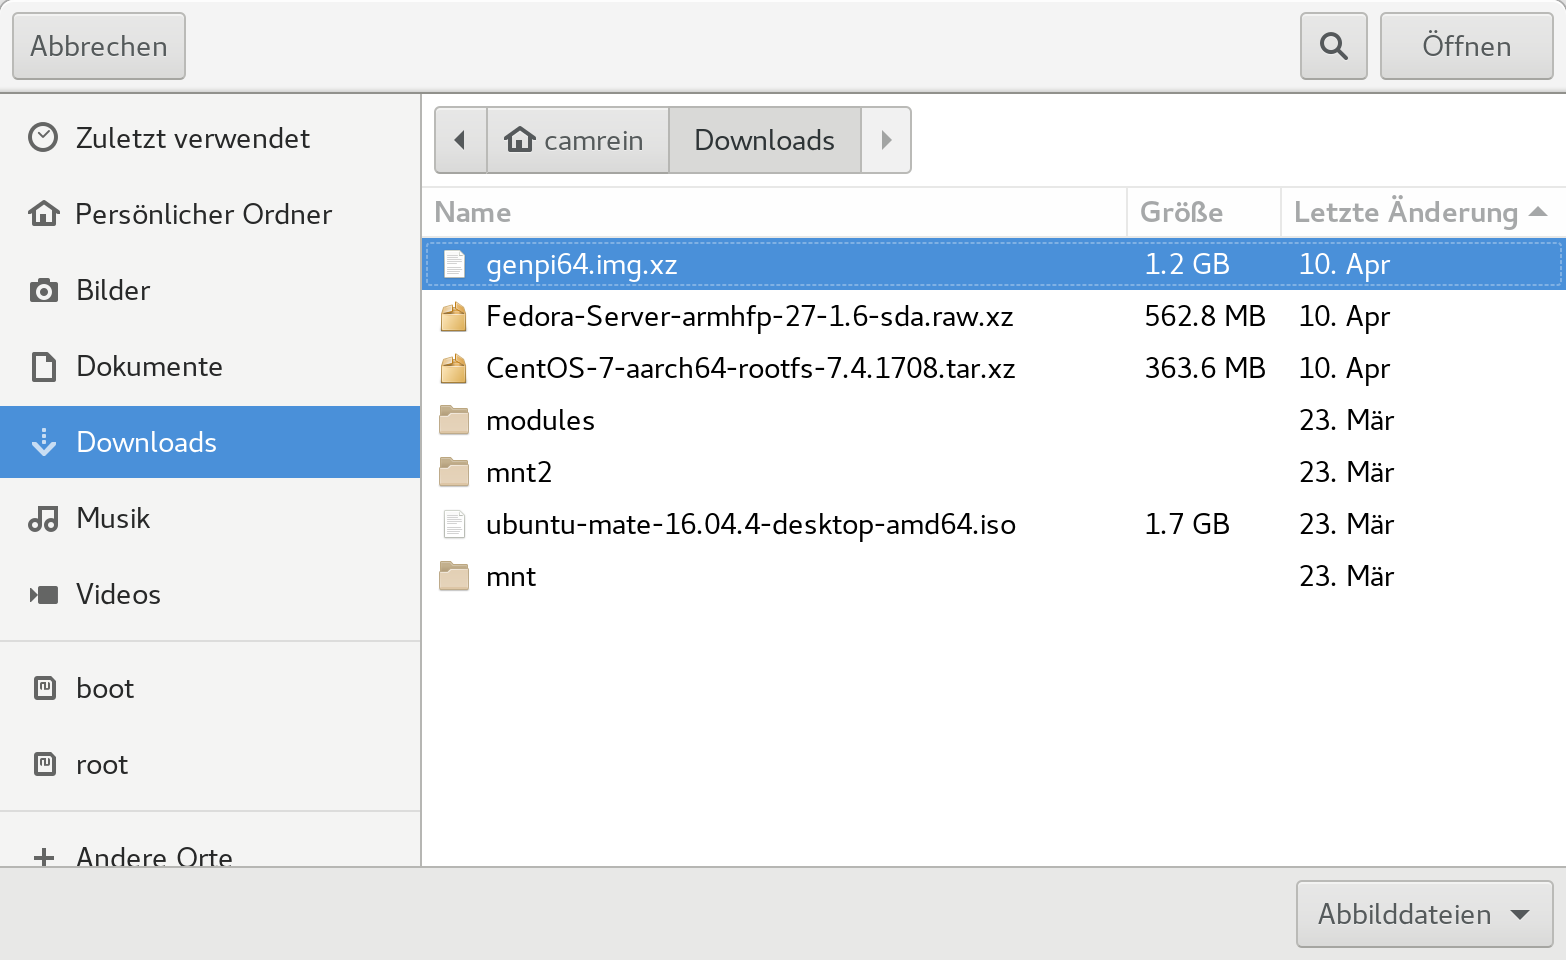
\includegraphics[scale=0.2]{Bilder/fmw2.png}
	\caption{FMW: Archiv auswählen}
\end{figure}
\begin{figure}[H]
	\centering
	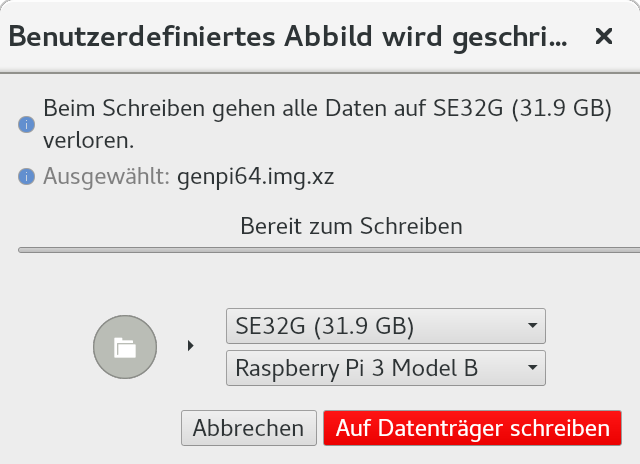
\includegraphics[scale=0.3]{Bilder/fmw3.png}
	\caption{FMW: Abbild schreiben}
\end{figure}
3. Durch das Schreiben des Archivs wurden zwei Partitionen (boot \& rootfs) auf der SD Karte erstellt. Diese werden wiefolgt ausgelesen:
\begin{lstlisting}
[camrein@wifibridge ~]\$ lsblk
NAME MAJ:MIN RM SIZE RO TYPE MOUNTPOINT
sda 8:0 0 238.5G 0 disk 
-sda1 8:1 0 200M 0 part /boot/efi
-sda2 8:2 0 1G 0 part /boot
-sda3 8:3 0 237.3G 0 part 
--fedora-root 253:0 0 50G 0 lvm /
--fedora-swap 253:1 0 7.8G 0 lvm [SWAP]
--fedora-home 253:2 0 179.5G 0 lvm /home
mmcblk0 179:0 0 29.7G 0 disk}
-mmcblk0p1 179:1 0 43.1M 0 part /run/media/camrein/boot
-mmcblk0p2 179:2 0 29.7G 0 part /run/media/camrein/rootfs
[camrein@wifibridge ~]\$
\end{lstlisting}
4. Die Dateisystem Partition muss mit der von CentOS überschrieben werden. Dazu wird die Partition auf dem Linux Client angehängt. Bei Schritt 5-7 wird überprüft ob die Partition wirklich leer ist.
\begin{lstlisting}
[root@wifibridge Downloads]# mkdir mnt
[root@wifibridge Downloads]# mount /dev/mmcblk0p2 mnt
[root@wifibridge Downloads]# cd mnt
[root@wifibridge mnt]# rm -rf *
[root@wifibridge mnt]# ls -lrtha
drwxr-xr-x. 5 camrein camrein 20K 15. Mai 17:39 ..
drwxr-xr-x. 2 root root 4.0K 16. Mai 17:58 .
\end{lstlisting}

Die Dateisystem Partition ist nun leer und kann mit der von CentOS überschrieben werden. \newline
5. Das Dateisystem aus dem offiziellen Centos Repository\footnote{\url{http://mirror.centos.org/altarch/7.4.1708/isos/aarch64/CentOS-7-aarch64-rootfs-7.4.1708.tar.xz}} beziehen. \newline
6. Die geleerte Partition wird nun mit dem Dateisystem von Centos7.4 überschrieben, zugleich soll bei Schritt 2 überprüft werden, ob die Daten wirklich auf die Partition geschrieben wurden.
\begin{lstlisting}
[root@wifibridge mnt]# tar --numeric-owner -xpJf ../CentOS-7-aarch64-rootfs-7.4.1708.tar.xz
[root@wifibridge mnt]# ls -lrtha
insgesamt 84K
drwxr-xr-x. 2 root root 4.0K 23. Nov 2016 srv
drwxr-xr-x. 2 root root 4.0K 23. Nov 2016 opt
drwxr-xr-x. 2 root root 4.0K 23. Nov 2016 mnt
drwxr-xr-x. 2 root root 4.0K 23. Nov 2016 media
drwxr-xr-x. 2 root root 4.0K 23. Nov 2016 home
drwxr-xr-x. 2 root root 4.0K 12. Sep 2017 dev
drwxr-xr-x. 2 root root 4.0K 12. Sep 2017 proc
drwxr-xr-x. 2 root root 4.0K 12. Sep 2017 run
drwxr-xr-x. 2 root root 4.0K 12. Sep 2017 sys
lrwxrwxrwx. 1 root root 7 12. Sep 2017 bin -> usr/bin
lrwxrwxrwx. 1 root root 8 12. Sep 2017 sbin -> usr/sbin
lrwxrwxrwx. 1 root root 9 12. Sep 2017 lib64 -> usr/lib64
lrwxrwxrwx. 1 root root 7 12. Sep 2017 lib -> usr/lib
drwxr-xr-x. 13 root root 4.0K 12. Sep 2017 usr
drwxr-xr-x. 19 root root 4.0K 12. Sep 2017 var
dr-xr-xr-x. 17 root root 4.0K 12. Sep 2017 .
drwxr-xr-x. 82 root root 4.0K 12. Sep 2017 etc
dr-xr-xr-x. 3 root root 4.0K 12. Sep 2017 boot
drwxrwxrwt. 7 root root 4.0K 12. Sep 2017 tmp
dr-xr-x---. 2 root root 4.0K 12. Sep 2017 root
drwxr-xr-x. 5 camrein camrein 20K 15. Mai 17:39 ..
[root@wifibridge mnt]#
\end{lstlisting}

Die SD Karte kann nun mit den RPI's verwendet werden. Diese starten jeweils mit dem Hostnamen centos.


\subsection{RPI für den Netzwerkboot vorbereiten}
Für das Vorbereiten der Clients für den Netzwerkboot wurde der Guide NETWORK BOOT YOUR RASPBERRY PI von raspberrypi.org\footnote{\url{https://www.raspberrypi.org/documentation/hardware/raspberrypi/bootmodes/net\_tutorial.md}} verwendet. Die RPI's werden wie folgt vorbereitet:

1. Die config.txt Datei im /boot Verzeichnis benötigt einen OTP Eintrag, dieser sagt aus, dass das RPI ohne SD Karte nach einem Betriebssystem anfragen soll. 
\begin{lstlisting}
echo program_usb_boot_mode=1 | sudo tee -a /boot/config.txt
\end{lstlisting}
2. RPI neustarten \newline
3. Prüfen ob die Änderung aktiv ist
\begin{lstlisting}
vcgencmd otp_dump | grep 17:
\end{lstlisting}
Erwartetes Ergebnis:
\begin{lstlisting}
17:3020000a
\end{lstlisting}
4. Den Eintrag in der /boot/config.txt wieder entfernen\newline
\textbf{MAC-Adressen auslesen}\newline
Um Zeit zu sparen können alle MAC-Adressen der RPI's während der Vorbereitung der Clients auf den Netzwerkboot ausgelesen werden.\newline
5. nmap Scan auf die IP Range 192.168.1.0-255 von einem Linux Client aus durchführen.
\begin{lstlisting}
	  nmap -sP 192.168.1.0/24  
\end{lstlisting}
Erwartetes Ergebnis für ein RPI:
\begin{lstlisting}
	  Nmap scan report for centos.home (192.168.1.11)
	  Host is up (0.00055s latency).
	  MAC Address: B8:27:EB:32:39:A7 (Raspberry Pi Foundation)   
\end{lstlisting}

Die Vorbereitung der RPI(Computenodes) ist somit abgeschlossen und es kann mit der Installation des Managementnode fortgefahren werden.

\subsection{Hostname und IP der MAC Adresse zuweisen}
über http://internetbox/ wird die IP Adresse sowie der Hostname der MAC Adresse der RPI's zugewiesen. Alle jemals angeschlossenen Geräte werden unter der Geräteliste aufgelistet. Dort können ebenfalls die Hostnamen den Geräten zugewiesen werden.

\begin{figure}[H]
	\centering
	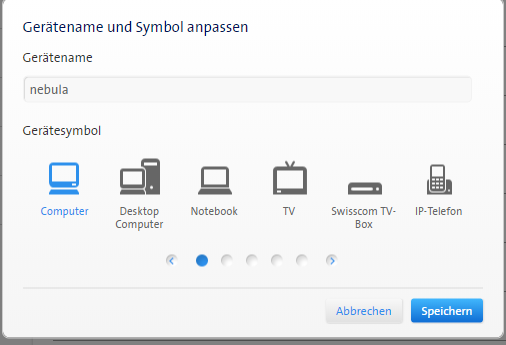
\includegraphics[scale=0.8]{Bilder/hostnamen_mac_edit.png}
	\caption{Hostnamen editieren}
\end{figure}
\begin{figure}[H]
	\centering
	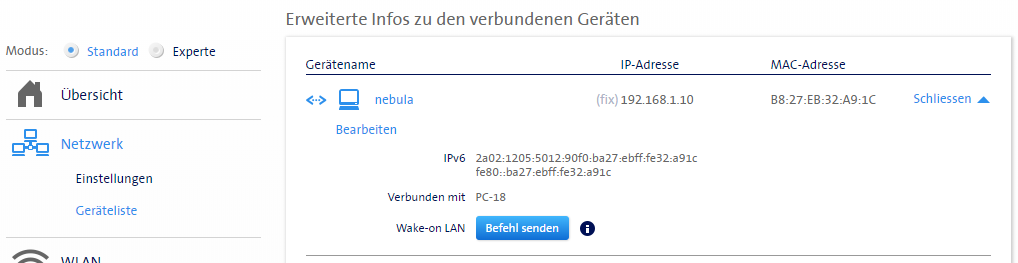
\includegraphics[scale=0.6]{Bilder/hostnamen_mac_overview.png}
	\caption{Übersicht der Hostnamen Zuweisung}
\end{figure}

Die fixe IP Adresse wird unter den Netzwerkeinstellungen des Routers direkt vorgenommen. Hierbei kann den bereits erkannten und definierten RPI's per Hostname eine IP zugewiesen werden.
\begin{figure}[H]
	\centering
	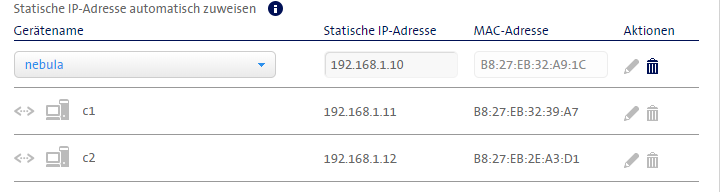
\includegraphics[scale=0.8]{Bilder/ip_mac_edit.png}
	\caption{Statische IP vergeben}
\end{figure}